\documentclass[a4paper,12pt]{article}
\usepackage{amsmath,amssymb,amsfonts,amsthm}
\usepackage{tikz}
\usepackage [utf8x] {inputenc}
\usepackage [T2A] {fontenc} 
\usepackage[russian]{babel}
\usepackage{cmap} 
\usepackage{ gensymb }
% Так ссылки в PDF будут активны
\usepackage[unicode]{hyperref}
\usepackage{ textcomp }
\usepackage{indentfirst}

% вы сможете вставлять картинки командой \includegraphics[width=0.7\textwidth]{ИМЯ ФАЙЛА}
% получается подключать, как минимум, файлы .pdf, .jpg, .png.
\usepackage{graphicx}
% Если вы хотите явно указать поля:
\usepackage[margin=1in]{geometry}
% Или если вы хотите задать поля менее явно (чем больше DIV, тем больше места под текст):
% \usepackage[DIV=10]{typearea}

\usepackage{fancyhdr}

\newcommand{\bbR}{\mathbb R}%теперь вместо длинной команды \mathbb R (множество вещественных чисел) можно писать короткую запись \bbR. Вместо \bbR вы можете вписать любую строчку букв, которая начинается с '\'.
\newcommand{\eps}{\varepsilon}
\newcommand{\bbN}{\mathbb N}
\newcommand{\dif}{\mathrm{d}}

\newtheorem{Def}{Определение}


\pagestyle{fancy}
\makeatletter % сделать "@" "буквой", а не "спецсимволом" - можно использовать "служебные" команды, содержащие @ в названии
\fancyhead[L]{\footnotesize Оптика}%Это будет написано вверху страницы слева
\fancyhead[R]{\footnotesize ФМХФ МФТИ}
\fancyfoot[L]{\footnotesize \@author}%имя автора будет написано внизу страницы слева
\fancyfoot[R]{\thepage}%номер страницы —- внизу справа
\fancyfoot[C]{}%по центру внизу страницы пусто

\renewcommand{\maketitle}{%
	\noindent{\bfseries\scshape\large\@title\ \mdseries\upshape}\par
	\noindent {\large\itshape\@author}
	\vskip 2ex}
\makeatother
\def\dd#1#2{\frac{\partial#1}{\partial#2}}


\title{4.3.1 \\ Изучение дифракции света}
\author{Егор Берсенев} 
\date{9 февраля 2017 г.}

\begin{document}
	\maketitle
	\section{Цель работы}
		Исследование явления дифракции Френеля и Фраунгофера на щели, изучить влияние на разрешающую способность оптических инструментов.
	\section{Оборудование}
		Оптическая скамья, ртутная лампа, монохроматор, щели с регулируемой шириной, рамка с вертикальной нитью, двойная щель, микроскоп на поперечных салазках с микрометрическим винтом, зрительная труба.
	
	\section{Теоретическое введение}
	\subsection{Дифракция Френеля}
		Схема установки для наблюдения дифракции Френеля на щели представлена на рис. 1. Световые лучи освещают щель $S_2$ и испытывают на ней дифракцию. Дифракционная картина рассматривается с помощью микроскопа $M$, сфокусированного на плоскость наблюдения $\text{П}$. 
		
		Щель $S_2$ освещается параллельным пучком монохроматического света с помощью коллиматора, образованного объективом $O_1$, и щелью $S_1$, находящейся в его фокусе. На щель $S_1$ сфокусировано изображение спектральной линии, выделенной из спектра ртутной лампы при помощи монохроматора, в котором используется призма прямого зрения. 
		
		\begin{figure}[h!]
			\label{fren}
			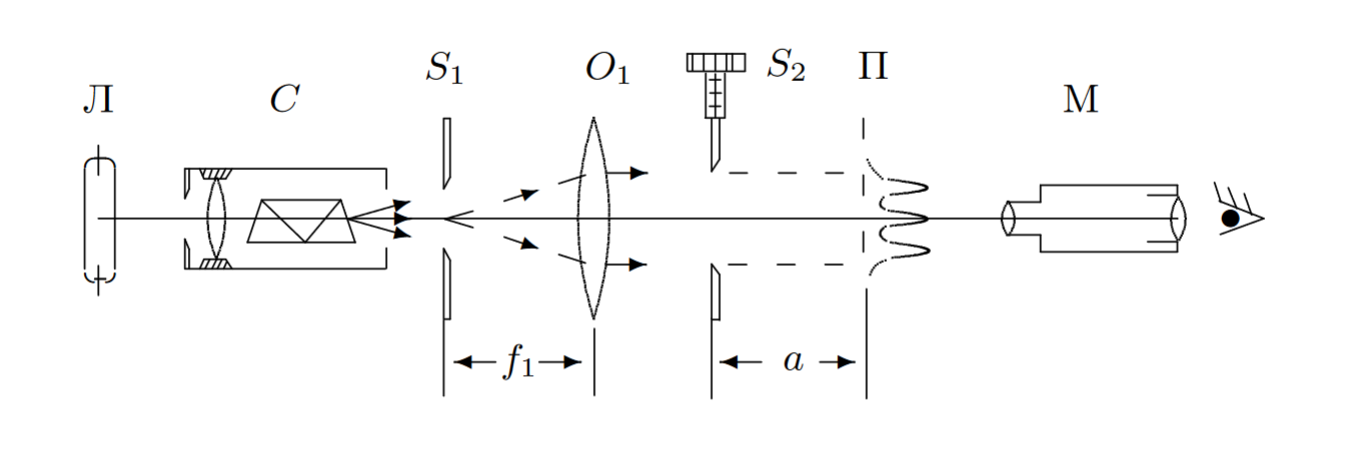
\includegraphics[width = 0.7\linewidth]{fren}
			\centering
			\caption{Схема установки для наблюдения дифракции Френеля}
		\end{figure}
		
		Распределение интенсивности  света в плоскости наблюдения проще всего рассчитывать с помощью зон Френеля. При освещении щели параллельным пучком лучей зоны Френеля представляют собой полоски, параллельные краям щели. Ширина $n$ зон Френеля определяется соотношением 
		\begin{equation}
			r_n = \sqrt{zn\lambda}
		\end{equation}
	
	\subsection{Дифракция Фраунгофера}
		На значительном удалении от щели, изображение размывается и возникает дифракционная картина, называемая дифракцией Фраунгофера. Для удобства наблюдения к вышеописанной схеме добавляется объектив $O_2$.
		
		\begin{figure}[h!]
			\label{fren}
			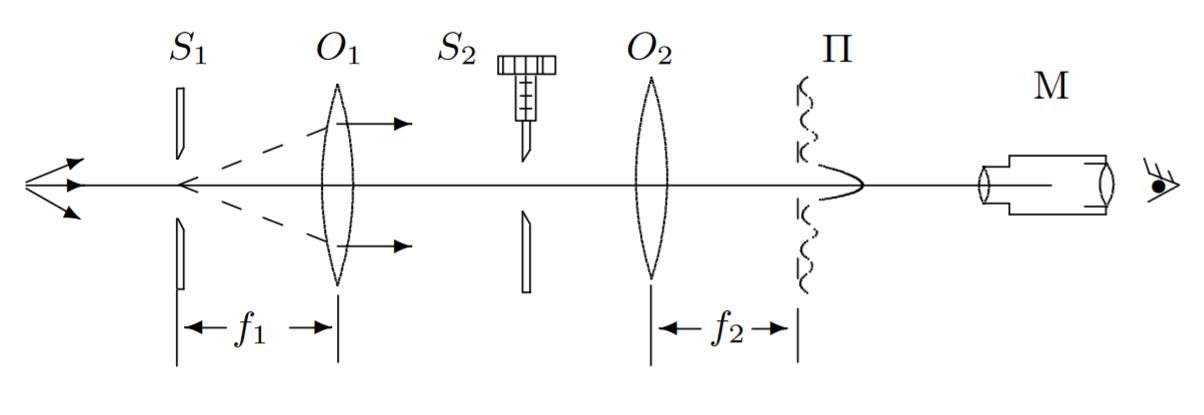
\includegraphics[width = 0.7\linewidth]{fraun}
			\centering
			\caption{Схема установки для наблюдения дифракции Фраунгофера}
		\end{figure}
		
		Дифракционная картина наблюдается здесь в фокальной плоскости объектива $O_2$. Каждому значению угла $\theta$ соответствует в этой плоскости точка, отстоящая на оптической оси на расстояние 
		\begin{equation}
			x = f_2\tan\theta = f_2\theta
		\end{equation}
		
		Поскольку объектив дополнительной разности хода не вносит, в его фокальной плоскости наблюдается неискаженная дифракционная картина Фраунгофера.
		
		В центре поля зрения наблюдается максимум. При малых углах положение минимумов определяется из:
		\begin{equation}
			b\theta = m\lambda \Leftrightarrow x_m b = f\lambda f_2
		\end{equation}
		
		\subsection{Влияние дифракции на разрешающую способность}
			Линзы $O_1$ и $O_2$ в отсутствие щели $S_2$ создают в плоскости $\text{П}$ изображение щели $S_1$ и это изображение рассматривается в микроскоп. Таким образом, установку можно рассматривать как оптический инструмент для получения изображения предмета. Если перед линзой $O_2$ расположить щели, то изображение объекта будет искажено дифракцией на щели $S_2$. Чем меньше ширина щели, тем сильнее искажение. Качественной характеристикой искажений может служить минимальное угловое расстояние $\varphi_{min}$ между объектами, которые воспринимаются как раздельные.
		
		\begin{figure}[h!]
			\label{fren}
			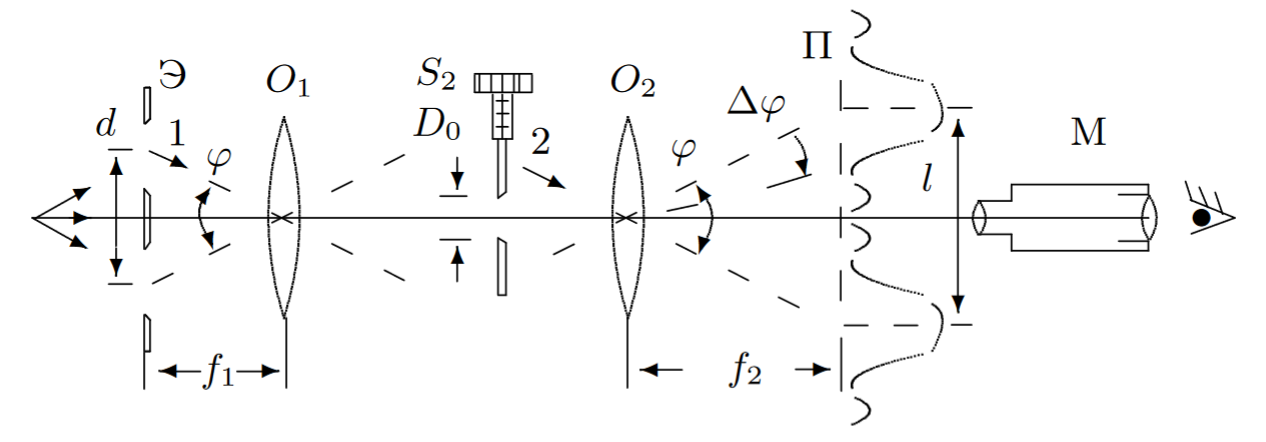
\includegraphics[width = 0.7\linewidth]{razr}
			\centering
			\caption{Схема установки для наблюдения искажений в оптических приборах}
		\end{figure}
		
		Если поставить вместо щели $S_1$ экран с двумя узкими щелями, расстояние между которыми $d$. Тогда на щель будут	два параллельных пучка света, составляющих между собой угол $\varphi$, равный:
		\begin{equation}
			\varphi = \frac{d}{f_1}
		\end{equation}
		
		Параллельных лучи 1 и 2, проходящие через центры линз, определяют положения изображений двойной щели. Согласно законам геометрической оптики расстояние $l$ между изображениями щелей в плоскости П равно:
		\begin{equation}
			l = \varphi f_2 = d \cdot \frac{f}{f}
		\end{equation}
		а ширина $\Delta\varphi$ каждого изображения определяется дифракцией света на щели $S_2$. Когда полуширина дифракционного изображения превышает расстояние между изображениями, то по виду дифракционной картины трудно определить, представляет собой источник двойную или одинарную щель. Кроме того, разные люди по разному различают предел, при котором изображения различимы. Поэтому чаще всего используется критерий Релея: изображения считаются различными, когда максимум одного дифракционного пятна совпадает с минимумом другого, а в нашей установке --- когда угловая полуширина дифракционного изображения $\frac{\lambda}{D_0}$ совпадает с угловым расстоянием $\varphi = \frac{l}{f_2}$ между изображениями отдельных щелей.
				
		
		\section{Экспериментальная часть}
		\subsection{Дифракция Френеля}
		
		Построим график зависимости $2z_n(n)$.
		
		\begin{figure}[h!]
			\label{pfren}
			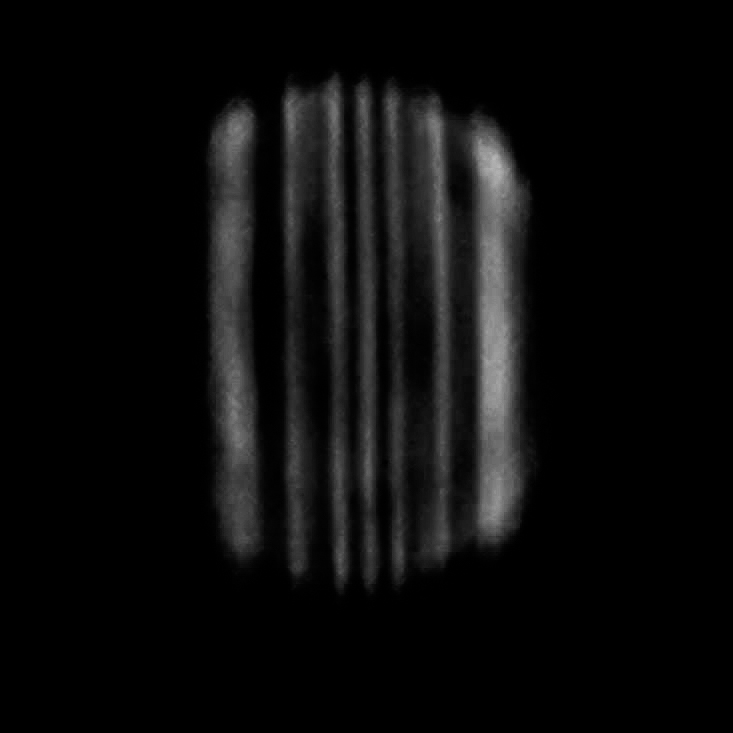
\includegraphics[width = 0.5\linewidth]{fr}
			\centering
			\caption{Дифракционная картина}
		\end{figure}
		
		\begin{figure}[h!]
			\label{gfren}
			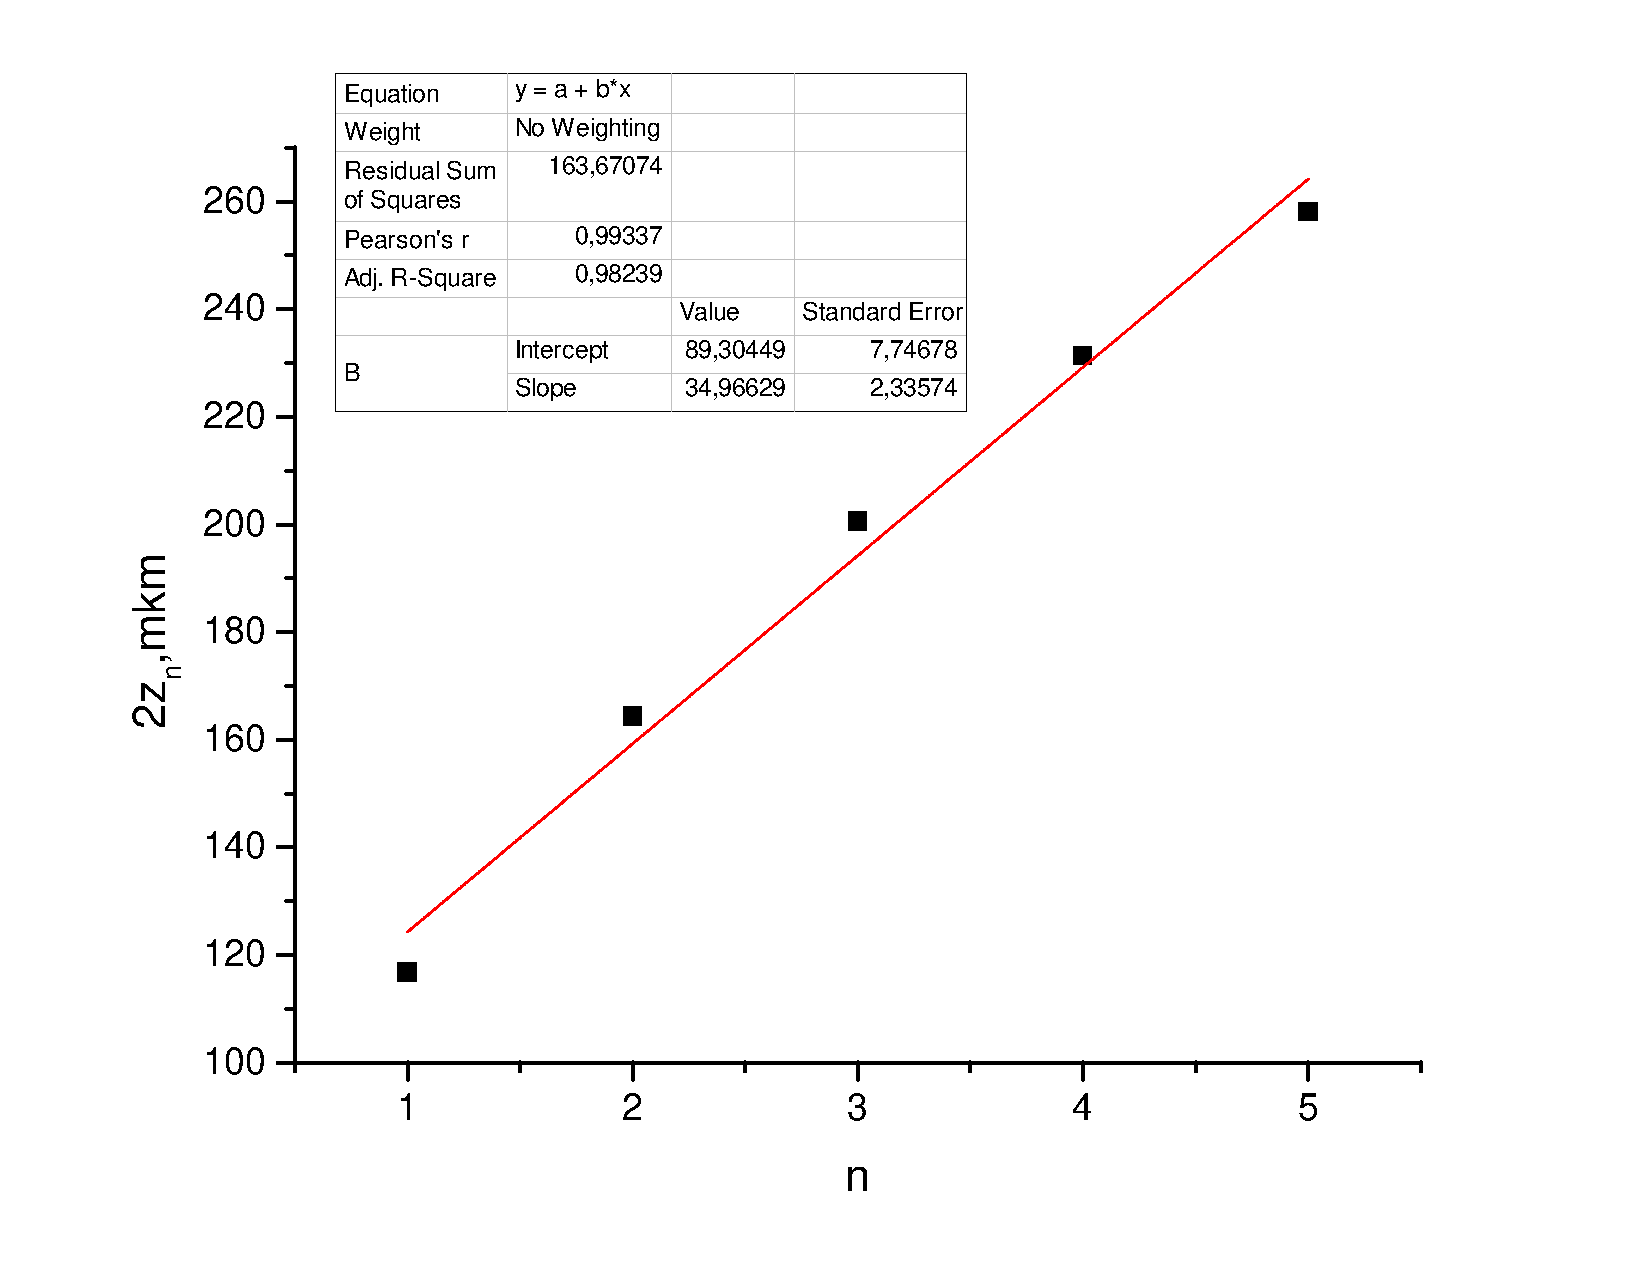
\includegraphics[width = 0.85\linewidth]{gfren}
			\centering
			\caption{$2z_n(n)$}
		\end{figure}
		
		\begin{figure}[h!]
			\label{gfraun}
			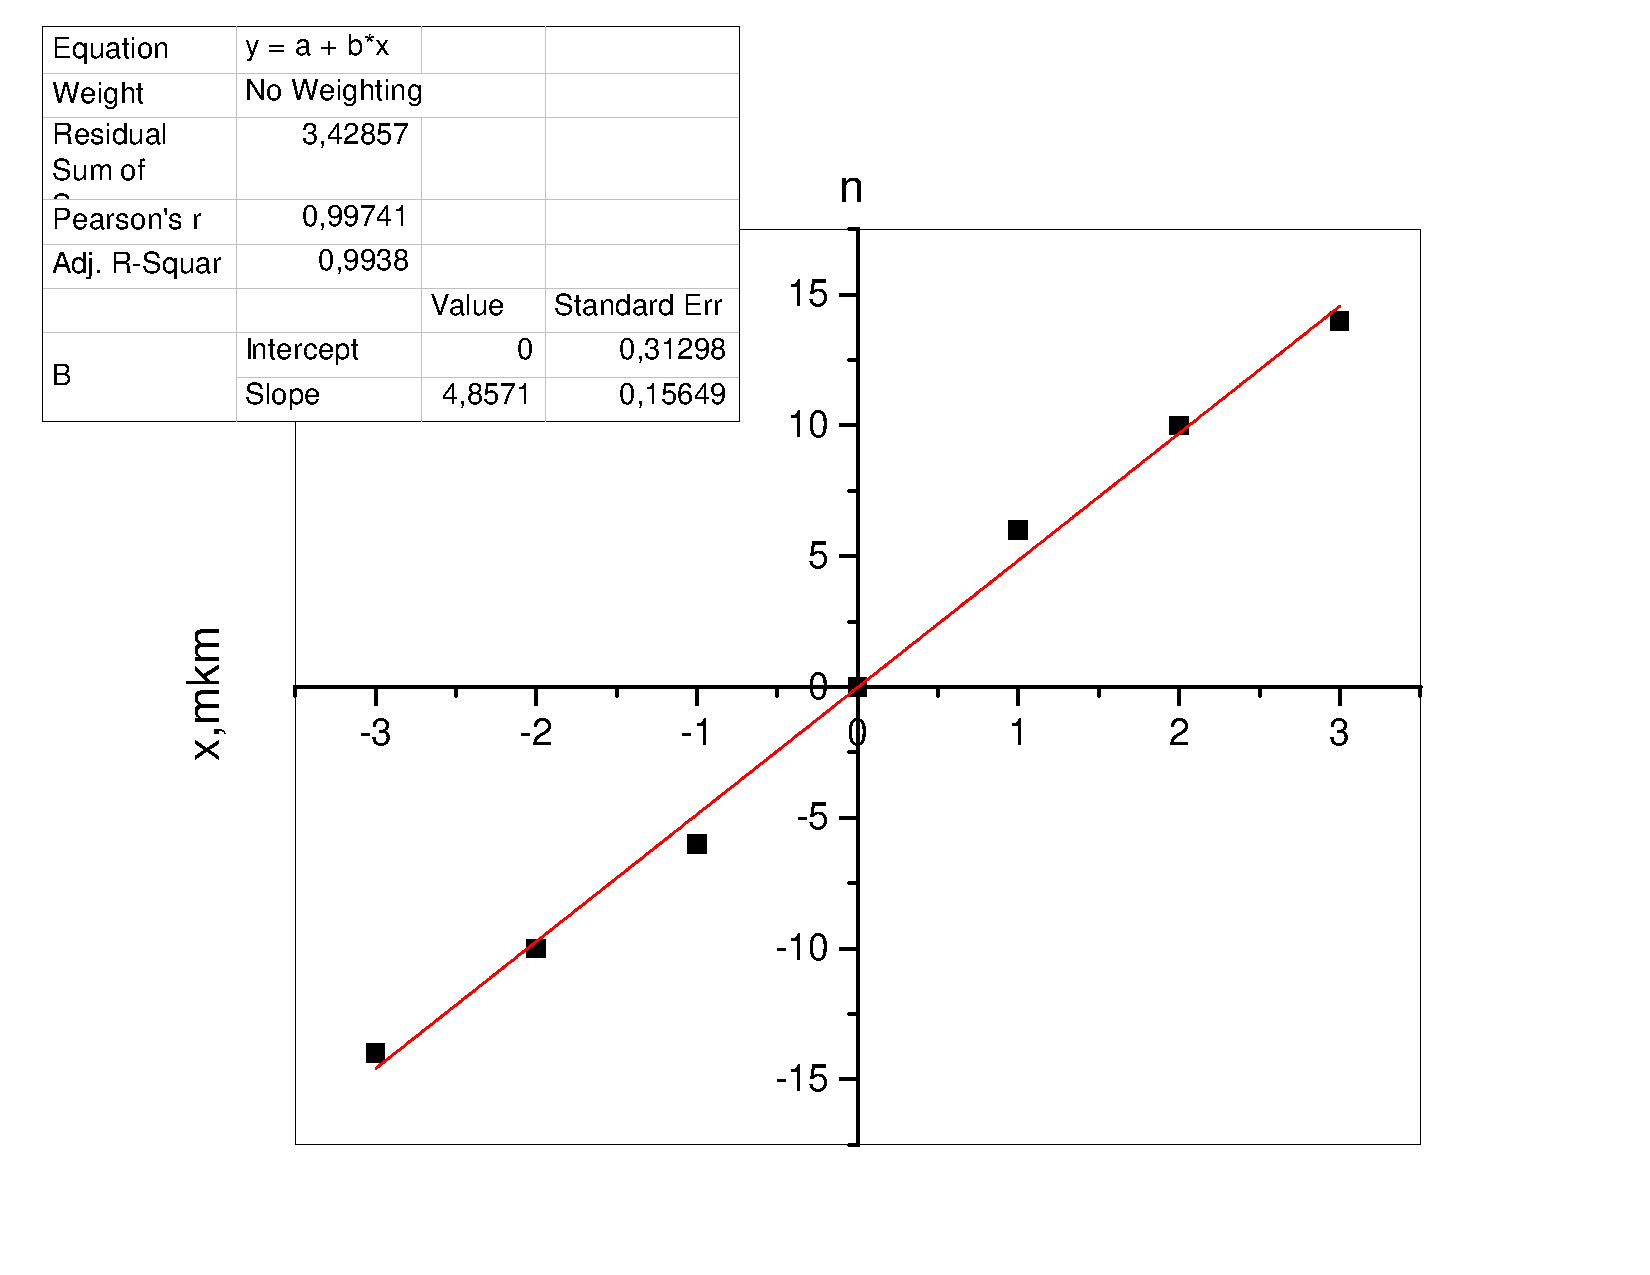
\includegraphics[width = 0.85\linewidth]{gfraun}
			\centering
			\caption{$x_n(n)$}
		\end{figure}
		
		
		
		\newpage
		
		\subsection{Дифракция Фраунгофера}
			Построим график зависимости координаты дифракционного минимума от номера полосы.
			
		Рассчитаем ширину щели $D = 135 \pm 7\,\text{мкм}$. Ширина щели, измеренная по микрометрическому винту: $D = 130 \pm 5 \,\text{мкм}$.
		
		\subsection{Измерения разрешающей способности}
		
		Измеренные с помощью микроскопа параметры двойной щели: $d=1.17$ мм, $b_l=0.23$ мм, $b_r=0.22$ мм
		
		Рассчитаем ширину щели: $b_0=\frac{\lambda f_1}{d}=58\pm 5\,\text{мкм}$.
		
		Подбирая ширину щели на глаз, получаем по микрометрическому винту $b_0 = 75 \pm 5 \,\text{мкм}$
		
		\section{Вывод}
		В проделанной работы была исследована дифракция Френеля, Фраунгофера на одной и двух щелях. Дифракцию Фраунгофера на двух щелях не удалось изучить подробно по причине слишком узких и размытых дифракционных полос.
\end{document}


